%; whizzy document
% latex beamer presentation.
% platex, latex-beamer $B$G%3%s%Q%$%k$9$k$3$H$rA[Dj!#(B 

%     Tokyo Debian Meeting resources
%     Copyright (C) 2006 Junichi Uekawa

%     This program is free software; you can redistribute it and/or modify
%     it under the terms of the GNU General Public License as published by
%     the Free Software Foundation; either version 2 of the License, or
%     (at your option) any later version.

%     This program is distributed in the hope that it will be useful,
%     but WITHOUT ANY WARRANTY; without even the implied warranty of
%     MERCHANTABILITY or FITNESS FOR A PARTICULAR PURPOSE.  See the
%     GNU General Public License for more details.

%     You should have received a copy of the GNU General Public License
%     along with this program; if not, write to the Free Software
%     Foundation, Inc., 51 Franklin St, Fifth Floor, Boston, MA  02110-1301 USA

% $B<B9T=gHV(B
% sudo  ~/bin/usb-macbook-ir.c &
% real presentation (shell-command (concat "DISPLAY=:0.1 xpdf -fullscreen " (replace-regexp-in-string "tex$" "pdf"(buffer-file-name)) "&"))
% DISPLAY=:0.1 xpdf -fullscreen 

\documentclass[cjk,dvipdfm,14pt]{beamer}
% 14 seems like the max relevant value 
\usetheme{Warsaw}
\usepackage{fancybox}%SBox

%  preview (shell-command (concat "xpdf " (replace-regexp-in-string "tex$" "pdf"(buffer-file-name)) "&"))
%  presentation (shell-command (concat "xpdf -fullscreen " (replace-regexp-in-string "tex$" "pdf"(buffer-file-name)) "&"))


%http://www.naney.org/diki/dk/hyperref.html
%$BF|K\8l(BEUC$B7O4D6-$N;~(B
\AtBeginDvi{\special{pdf:tounicode EUC-UCS2}}
%$B%7%U%H(BJIS$B7O4D6-$N;~(B
%\AtBeginDvi{\special{pdf:tounicode 90ms-RKSJ-UCS2}}

\title{$B??$N(BLinux Kernel $B8~$1%7%'%k(B}
\subtitle{LL GONG @ LL RING 2006}
\author{$B>e@n(B $B=c0l(B \\dancer@debian.org\\ Debian Project}
\date{2006$BG/(B8$B7n(B26$BF|(B}
\logo{
\includegraphics[width=8cm]{image200607/openlogo-light.eps}}

% $B;0BrLdBjMQ(B
\newcounter{santakucounter}
\newcommand{\santaku}[5]{%
\addtocounter{santakucounter}{1}
\frame{\frametitle{$BLdBj(B\arabic{santakucounter}. #1}
%$BLdBj(B\arabic{santakucounter}. #1
\begin{minipage}[t]{0.7\hsize}
 \begin{itemize}
 \item A #2\\
 \item B #3\\
 \item C #4\\
 \end{itemize}
\end{minipage}
}
\frame{\frametitle{$BLdBj(B\arabic{santakucounter}. #1}
%$BLdBj(B\arabic{santakucounter}. #1
\begin{minipage}[t]{0.7\hsize}
\begin{itemize}
\item A #2\\
\item B #3\\
\item C #4\\
\end{itemize}
\end{minipage}
\begin{minipage}[t]{0.2\hsize}
$BEz$($O(B:


\vspace{1cm}

{\huge \hspace{1cm}#5}
\end{minipage}}
}


\begin{document}
\frame{\titlepage{}}

\begin{frame}
\frametitle{$B%"%8%'%s%@(B}
\begin{center}
 \begin{minipage}{0.5\hsize}
 \begin{itemize}
 \item $B;~BeGX7J(B
 \item $B%D!<%k>R2p(B
 \item $B<B1i(B
 \end{itemize}
 \end{minipage}
\end{center}
\end{frame}

\section{$B;~BeGX7J(B}

\subsection{UNIX$B$N4pK\%D!<%k(B}
\begin{frame}
\frametitle{UNIX$B$N4pK\%D!<%k(B}

$B%7%'%k$,4pK\$N%9%/%j%W%H8@8l(B ($B85AD(BLL?)

C $B$O%7%9%F%`3+H/8@8l(B

\end{frame}

\subsection{C$B8@8l(B}

\begin{frame}
\frametitle{shell$B$H$O(B}
\begin{itemize}[<+->]
 \item shell $B$O$J$s$@$+8@8l;EMM$,@)8B$5$l$F$$$F;H$$$K$/$$(B
 \item C $B$O$J$s$@$+5$7Z$K;H$($J$$$N$G(BLL$B$8$c$J$$$h!)(B
\end{itemize}
\end{frame}

\begin{frame}
\frametitle{C$B8@8l$N;~Be$NN.$l(B}
 \begin{itemize}[<+->]
  \item Linux Kernel $B$N%3!<%G%#%s%0$J$II,MW$J>lLL$OB?$$(B
  \item emacs buffer $B$G$9$3$7$E$D$?$a$7$J$,$i%3!<%I$,$+$1$k8@8l$,$&$i$d$^$7$$(B
  \item $BB>$N$[$H$s$I$N8@8l$O%$%s%?%W%j%?E*$KF0:n$9$k%$%s%?%U%'!<%9(B
	$B$,$"$j!"%3%s%Q%$%k!&%j%s%/$N<j=g$r>JN,$G$-$k$N$K(B
  \item $BB>$N$[$H$s$I$N8@8l$K$OBPOC%$%s%?%U%'!<%9$,$"$j!"(B
	$B$?$a$7$J$,$i%3!<%I$,=q$1$k$N$K(B
  \item $B$b$7$+$7$F$"$^$jN.9T$C$F$$$J$$!)(B
 \end{itemize}
\end{frame}

\begin{frame}
\frametitle{C$B8@8l$N;~Be$NN.$l(B}
 $B8+$?L\$@$1$G$b(BLL$BE*$K$7$?$$(B!
\end{frame}

\subsection{shell$B$X$N4|BT(B}

% $B@h?M$N0dJ*$OB8:_$9$k$,!"$=$l$,M-8z$K3hMQ$5$l$F$$$J$$$>!#(B

\begin{frame}
\frametitle{$B%7%'%k3F<o(B}
\begin{minipage}[t]{0.3\hsize}
   \onslide<1->sh\\
   \onslide<2->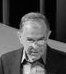
\includegraphics[width=1\hsize]{image200609/bourne.png}
\end{minipage}
\begin{minipage}[t]{0.3\hsize}
   \onslide<1->csh\\
   \onslide<3->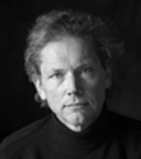
\includegraphics[width=1\hsize]{image200609/billjoy.png} 
\end{minipage}
\begin{minipage}[t]{0.3\hsize}
   \onslide<1->ksh\\
   \onslide<4->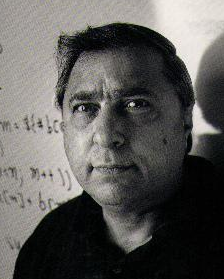
\includegraphics[width=1\hsize]{image200609/korn.png}
\end{minipage}

\begin{center}
    \onslide<5-> C$B$NIa5Z$N$?$a$N3WL?I,MW(B
\end{center}
\end{frame}

\section{$B%D!<%k>R2p(B}

\begin{frame}
\frametitle{$B%D!<%k>R2p(B}

\begin{center}
 \begin{minipage}{0.5\hsize}
 \begin{itemize}
 \item binfmtc
 \item realcsh
 \item realksh
 \end{itemize}
 \end{minipage}
\end{center}

\end{frame}

\subsection{binfmtc}

\begin{frame}
\frametitle{LL$B2=(B}
\begin{itemize}[<+->]
 \item C$B$r%9%/%j%W%H8@8l$_$?$$$K;H$$$?$$(B!
 \item $B8+$?L\$@$1%9%/%j%W%H8@8lIw(B
\end{itemize}
\end{frame}

\begin{frame}
\includegraphics[width=0.7\hsize]{image200609/binfmtc.eps}
\end{frame}

\begin{frame}{C$B$r(BLL$B$C$]$/;H$$$?$$(B!}

Linux Kernel $B$N5!G=$rMQ$$$F(BC$B8@8l$N%=!<%9$r%9%/%j%W%H$H$7$F<B9T(B

{\tt \small
\fbox{\begin{minipage}{1\hsize}
  {\bf coreduo:demo$>$} ./upaccho2.c\\
 upaccho2-webservice.c: In function 'http\_initiate\_webserver':\\
 upaccho2-webservice.c:194: warning: pointer targets in passing argument 3 of 'accept' differ in signedness\\
 Please specify the port as the command-line parameter\\
\end{minipage}}}

\hfill{} \onslide<2->... $B0l1~%"%W%j%1!<%7%g%s$OF0$$$F$$$k$,$J$s$@$+7Y9p$O$G$F$$$k!#(B
\end{frame}

\begin{frame}{C$B$r(BLL$B$C$]$/;H$$$?$$(B!}

$B=$@5$7$FB(<B9T(B

{\tt \small
\fbox{\begin{minipage}{1\hsize}
  {\bf coreduo:demo$>$} ./upaccho2.c\\
 Please specify the port as the command-line parameter\\
\end{minipage}}}

\hfill{} \onslide<2->... $B$J$s$@$+(BLL!
\end{frame}

\subsection{realcsh}
\begin{frame}
\begin{itemize}[<+->]
 \item C$B8@8l$r%7%'%k$H$7$F;H$$$?$$!*(B
 \item csh$B$C$F$"$k$s$@$1$I!"$J$s$+0c$&$h$M!)(B
\end{itemize}
\end{frame}

\begin{frame}

{\small \tt 
\fbox{\begin{minipage}{1\hsize}
{\bf coreduo:\~{}$>$} while (1) { printf ( "\%s$\backslash$n", "hello"); }\\
while: Expression Syntax.
\end{minipage}
}}

\hfill{}\onslide<2->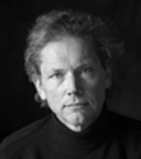
\includegraphics[width=0.3\hsize]{image200609/billjoy.png} 

\end{frame}

\begin{frame}

{\small \tt 
\fbox{\begin{minipage}{1\hsize}
{\bf coreduo:\~{}$>$} realcsh.c\\
{\bf REAL csh:} while (1) { printf ( "\%s$\backslash$n", "hello"); }\\
hello\\
hello\\
hello\\
hello\\
hello\\
.\\
.
\end{minipage}
}}
\end{frame}


\begin{frame}
\includegraphics[width=0.8\hsize]{image200609/realcsh.eps}
\end{frame}

\subsection{realksh}

\begin{frame}
\begin{itemize}[<+->]
 \item C$B8@8l$O(BLinux Kernel$B$N3+H/$KMxMQ$9$k8@8l(B
 \item $B%3!<%I$O;n$7$J$,$i3+H/$7$?$$(B
 \item $B%7%'%k$,L5$$$HITJX$@!<(B
 \item $B$=$&$$$($P!"(Bksh$B$C$F$N$,$"$k(B
\end{itemize}
\end{frame}

\begin{frame}
\frametitle{ksh $B$C$F$J$s$G(B kernel $B$8$c$J$$$s$@(B?}  
\fbox{
\begin{minipage}{0.9\hsize}
{\tt \small
{\bf \$} uname -r \\
2.6.18-rc3dancer\\
{\bf \$} printk ("\%i$\backslash$n", (int) jiffies); \\
ksh: syntax error: `(' unexpected\\
}
\end{minipage}
}

\hfill{}\onslide<2->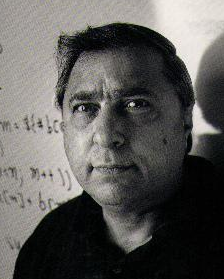
\includegraphics[width=0.3\hsize]{image200609/korn.png}

\end{frame}

\begin{frame}
\frametitle{ksh $B$C$F$J$s$G(B kernel $B$8$c$J$$$s$@(B?}
\fbox{
\begin{minipage}{0.9\hsize}
{\tt \small
{\bf REAL ksh: }$\sharp{}$include $<$linux/utsrelease.h$>$\\
REAL ksh: printk ("\%s$\backslash$n", UTS\_{}RELEASE); \\
  Building modules, stage 2.\\
KMSG: <4>2.6.18-rc3dancer\\
\\
{\bf REAL ksh: }printk ("\%i$\backslash$n", (int) jiffies);\\
  Building modules, stage 2.\\
KMSG: <4>5013786\\

}
\end{minipage}
}

\hfill{}\onslide<2->$B4A$J$i$3$&$$$&%7%'%k$,$h$$(B
\end{frame}

\begin{frame}
\includegraphics[width=0.7\hsize]{image200609/structure.eps}
\end{frame}

\section{$B<B1i(B}
\begin{frame}
\frametitle{$B<B1i(B}
\begin{itemize}
 \item jiffies $B$NI=<((B
 \item kernel version $B$NI=<((B
 \item BUG$B$NH/@8(B
% include <asm/bug.h> BUG()
\end{itemize}
\end{frame}

\section{$B$^$H$a(B}
\begin{frame}
\begin{center}
 \begin{minipage}{0.6\hsize}
 \begin{itemize}[<+->]
 \item LLGONG
 \item Lowlevel Language GONG 
 \item $BB>$N$d$D$i$N2<$r$f$1(B!
  \item (Debian) \texttt{apt-get install binfmtc} $B$G%$%s%9%H!<%k2DG=(B
 \end{itemize}
 \end{minipage}
\end{center}
\end{frame}

\end{document}
